\documentclass[a4paper,12pt]{paper}


% Set margins
\usepackage[hmargin=2cm, vmargin=2cm]{geometry}
\usepackage{setspace}
\onehalfspacing



% Language packages
\usepackage[utf8]{inputenc}
\usepackage[T1]{fontenc}
\usepackage[magyar]{babel}

% AMS
\usepackage{amssymb,amsmath}

% Graphic packages
\usepackage{graphicx}
\graphicspath{ {./kepek/} }

% Colors
\usepackage{color}
\usepackage[usenames,dvipsnames]{xcolor}

% Enumeration
\usepackage{enumitem}

\begin{document}

\begin{center}
   \large \textbf{Hangvezérelt aszisztens asztali környezetekhez}
\end{center}

\vskip 1cm

\section{Feladat}

Beszédfelismerés módszertanánk megismerése. A rejtett Markov modell és a dinamikus idővetemítés alkalmazásával hangminták elemzése. Hangjellemzők kinyerése. Gépi tanulási módszerek alkalmazásával modell betanítása minták alapján. Asztali környezeti műveletek végrehajtásának megvalósítása egyszerű vezényszavak segítségével. Elkészült alkalmazás használhatóságának tesztelése, eredmények értékelése.

\section{Hangfeldolgozási módszerek}

\subsection{Bevezetés}
% TODO: Leírni, hogy milyen célból, és nagyvonalakban hogy szokták feldolgozni.
A számítógépes nyelvészet több területet foglal magába, melyek a beszédfelismerés, beszédszintézis, elemzés(parsing), szemantikai elemezés, generálás és inferencia. Számítógépünk a nyelvet szövegként értelmezi melyek számkódok sorozata, ahol ezek a kódok betűket és írásjeleket képviselnek. A tároláson és megjelenítésen túl, a szövegben fel kell ismerni a nyelvi szerkezeteket. Természetes nyelvek esetén szabályszerűségekkel szembesülünk, melyeket értelmezni kell. Szavainknak és mondatainknak felismeréséhez megfelelő világismeretre van szükség.  \\\\A beszédfelismerés manapság már igen elterjedt funkció a mai rendszerekben, leginkább telefonunkban találkozhatunk vele. Számítógépes asztali környezetekhez is kapunk kész megoldásokat mint asszisztensek, például Microsoft Windows-nál Cortana, illetve macOS-nél Siri személyében, melyekkel interaktívan elvégezhetünk bizonyos tevékenységeket vagy valamilyen beszédfelismerő szoftvert használhatunk. Ezek zártkörű rendszerek, nem látunk bele hogyan működik. Vannak nyílt forráskódú rendszerek is, de komplex tervezésem és szakdolgozatom témája az, hogy a fent említett rendszerekhez hasonló, de egy nyílt forráskódú offline működő hangvezérelt asszisztenst készítsek. 

\subsection{Fogalmak, definíciók}

A beszédfelismerés több tudományterület eredményét kapcsolja össze, melyek a statisztikus mintaillesztés, a kommunikációelmélet, a jelfeldolgozás, a kombinatorikus matematika, a nyelveszét és egyebek. Ahhoz, hogy ezeket megismerjük, igencsak széleskörű ismeretek szükségesek. Ezek a rendszerek leegyszerűsítve minimum 3 elemből kell, hogy felépüljenek, melyek a következők: egy olyan bemeneti egység ami a jelfeldolgozásért felel, egy mintaillesztő egység, és egy dekóder ami nyelvmodell alapú feldolgozó egység. A beszédfelismerés röviden az alábbi módon zajlik le. Van egy személy akinek a beszédének hanghullámjait egy mikrofon segítségével analóg elektromos jellé , majd ezt követően, hogy számítógépünk tudja értelmezni digitális jellé alakítjuk. Ezután a számítógépünk egy adott  beszédfelismerő program segítségével meg adja az adott kifejezést és felhasználja azt.
\begin{figure}[h]

	\centering
	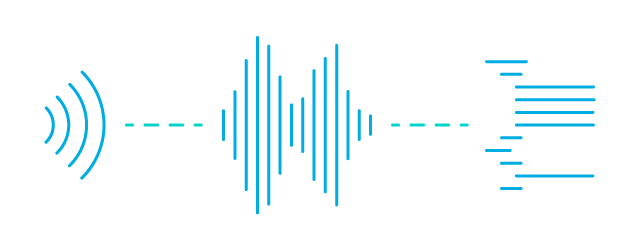
\includegraphics[width=0.7\textwidth]{amazonsr}
	\caption{A beszédfelismerés folyamata}
\end{figure}
\\Mielőtt még belemegyünk a rejtelmeibe ennek a tématerületnek, néhány alapvető fogalmat, definíciót tisztáznunk kell. A fizikai értelemben vett hang egy mechanikai rezgés, ami csak anyagi közegben terjedhet. Mindennapi életünkben hallott hang a levegő molekuláinak a hangforrástól kiinduló, egyre csillapodva tovaterjedő mechanikai rezgése. Azonban mechanikai rezgés nem csak levegőben, hanem egyéb rezgésre hajlamos rugalmas közegekben is létrejöhet. A hang tehát valamilyen rugalmas közegben terjedő mechanikai rezgéshullám, amely az élőlényekben hangérzetet kelt. 
\\Ahhoz, hogy egy közegben rezgés keletkezzen, szükség van egy adott nagyságú felületre, amely a körülette levő közeg részecskéit valamilyen mértékben megmozgatja. A rezgés erőssége a vivőközeggel közölt erő nagyságától és a felület terjedelmétől függ.
\\A hanghullám rugalmas közegben terjedő rezgés. A hullámterjedése közben a közegben valamilyen fizikai mennyiség változik(kitérés,nyomás,sűrűség). A közeg lehet szilárd, cseppfolyós, vagy légnemű halmazállapotú. Leggyakoribb hangtovábbító közeg a levegő. A hangforrás közelében  a rezgést továbbító levegő részecskéinek elmozdulása miatt nyomásingadozás jön létre, amely átterjed a szomszédos részecskékre ezáltal a levegőben tovaterjedő hanghullámok jönnek létre. 
\\Hangsebességen a hangrezgések közegben való terjedési sebességét értjük. A hangsebesség a közegre jellemző érték, amely csak a közeg sűrűségétől és rugalmasságától függ. A hangsebesség fizikai jele: c , egysége: méter/másodperc. A hang terjedési sebessége 15C hőmérsékletű levegőben 340 m/s.
\\A tiszta szinusos hangrezgés egyik fő jellemzője a másodpercenkénti rezgésszám vagy frekvencia. Ezt a hangrezgést tiszta hangnak nevezzük. Gyakorlatban viszont összetett hangok fordulnak elő, melyeknél a frekvencia általában nem értelmezhető, kivéve a periodikus hangrezgéseket, amelyek frekvenciáján az alapharmonikus frekvenciáját értjük.
\\A frekvencia egysége a hertz, jele Hz. 1 Hz frekvenciájú az a rezgés amelynek 1 másodperc alatt egy teljes periódusa játszódik le. Az amplitúdóval a szinuszos hangrezgés erősségét, azaz intenzitását jellemezhetjük. Egyetlen félperiódust vizsgálva az amplitúdó a rezgő részecske alaphelyzetétől mért legnagyobb kitérést jelenti. Minél nagyobb egy hangrezgés amplitúdója, annál nagyobb rezgési energiát képes közölni a vivőközeggel.
\\A gyakorlatban előforduló hangrezgések amplitúdója az idő és távolság függvényében soha nem állandó, hanem csökkenő jellegű. A hangrezgés amplitúdójának csökkenése a közeg mechanikai súrlódásával magyarázható. Az ilyen jellegű rezgéseket csillapított rezgéseknek nevezzük. Ahhoz, hogy a közeg egy meghatározott szakaszán csillapítatlan hangrezgéseket állítsunk elő a hangenergia veszteségeket állandóan pótolni kell.
\\ Tiszta hangnak nevezzük a tiszta szinusos hangrezgést, azaz azt a hangot amelynek spektrumában egyetlen vonal van. Gyakorlatban  azonban szinte kizárólag csak összetett hangokkal van dolgunk. Azokat a hangrezgéseket, amelyeknek frekvenciaspektrumában nemcsak egy, hanem több, egymástól különböző frekvenciájú komponensek találhatóak, összetett hangoknak nevezzük. Vannak periodikus és nemperiodikusak. 
\\A keltett hang magasságát mindig a frekvenciája határozza meg. A természetes hangforrások azonban az alaphangon kívül magasabb rezgésszámú hangösszetevőket is keltenek.
\\Ha a természetben csak tiszta hangok fordulnának elő, a különböző hangforrások hangját nem lehetne megkülönböztetni azonos magasságú hang keltése esetén. A hangnak van hangszínezete. A hangszínezet az alaphanghoz keveredő felhangok számától és erősségétől függ, és ugyanakkor független az összetevők fázis viszonyától. A hangszínezetet nagy mértékben meghatározza a hangforrás.
\\A hangforrás rezgő felülete mozgásba hozza a környezetében levő levegő molekuláit, amelyek a mozgás hatására sűrűsödnek, illetve ritkulnak azaz nyomásingadozás lép fel a levegőben. A rezgésbe hozott részecskék kitérése és a fellépő nyomásingadozás között meghatározott fizikai kapcsolat van. Ez a nyomásváltozás jelenti a hangingert, aminek erősségét hangerősségnek nevezzük. A hangerősség objektíven mérhető fizikai mennyiség, amely az élőlényekben szubjektív hangerősségérzetet kelt. A hangerősséget vagy hangnyomásban vagy intenzitásként fejezik ki, amit az egységnyi felületre jutó hangteljesítményben adják meg.
\\\\A következőkben az idő- és frekvenciatartománnyal kapcsolatos fogalmakról teszek egy rövid bemutatást.
\\Az analóg jel időben változó feszültség- (áram-) érték. Értelmezési tartománya a pozitív időtengely, értéktartománya folytonos - feszültség (áram). Az értéktartomány általában előre ismert és korlátos. 
\\A frekvencia vagy más néven spektrum egy (kör)frekvencia függvény, az analóg jel (időfüggvény), frekvencia-tartománybeli megfelelőjének (transzformáltjának) abszolút értéke.
\\A spektogram egy kétváltozós (idő és frekvencia) függvény. Egy hosszabb időfüggvényt időtartományokra (szeletekre) bontunk úgy, hogy kis egymásutáni időfüggvények sorozata adja ki az eredetit. Ezután mindegyik kis időfüggvényből készítünk egy frekvenciaspektrumot. A frekvenciaspektrumok egymásutánisága jelenti a spektrogramot.
\\A Fourier transzformáció: egy eljárás, amelynek segítségével az idő- és frekvenciatartományok közötti átmenet elvégezhető. Ha egy T periódusú analóg jel transzformációja a cél, akkor Fourier sorbafejtésről beszélünk. Ha analóg jelünk a periódikus, akkor a Fourier integrál módszert kell alkalmaznunk. Egy (analóg jel digitalizálásából eredő) számsor Fourier transzformációjára is van lehetőség, ekkor Diszkrét Fourier transzformációnak nevezett módszert (DFT) használunk, míg ennek gyorsított algoritmusa a gyors Fourier transzformáció (FFT).
\\A transzformációk eredménye egy w-tól függő komplex függvény F(w). Hangfeldolgozó programokban frekvenciaspektrum címén, általában ennek a függvénynek az abszolút értékét ábrázolják . A teljességhez hozzátartozna a komplex függvény fázisa is, azonban a fül csekély mértékű fázisérzékenysége miatt, ezt a legtöbb hangfeldolgozó eljárás elhanyagolja.
\\A szűrés egy frekvenciaspektrum módosító eljárás. Analóg jelünk eredeti spektrumát szűrők segítségével torzítjuk. Bizonyos frekvenciakomponenseket (tartományokat) kiemelünk (erősítünk), míg másokat elnyomunk. A szűrés célja a kellemesebb hanghatás elérésétől (szubjektív), az (objektív) mérési eredmények zajból való kihalászásáig igen sokrétű lehet. Szűrőzés eszközéül szintén több módszer közül válogathatunk. Szűrhetjük az analóg jelet közvetlenül analóg szűrők segítségével. Ezek lehetnek passzív, vagy aktív RLC szűrők. Az L,C elemek w -függő tulajdonságain alapulnak. Közvetett módon akkor szűrünk, amikor az analóg jelet előbb digitalizáljuk, majd ezen a számsoron végzünk különböző műveleteket úgy, hogy a módosított számsorból visszalakított analóg jel olyan legyen, mintha az eredetit szűrtük volna közvetlen módszerekkel.
\\Mintavételezés során a folytonos időfüggvényből D T időközönként értékeket, “mintákat” veszünk. Ezek továbbra is analóg értékek, viszont fontos bemeneti jeléül szolgálnak egy analóg-digitál átalakítónak. A mintavételezést ún. mintavevő és tartó áramkörök végzik. A mintavételi frekvencia kifejezi, hogy másodpercenként hány mintavétel történik.
\\A mintavételi törvény a következőt mondja ki: azt az időfüggvényt, amelynek frekvenciaspektrumában előforduló legmagasabb frekvenciájú komponens fmax értékű, legalább $fmv^{3}$ 2 fmax mintavételi frekvenciával kell mintavételeznünk. Pl. a zenei CD-kre rögzíteni kívánt legmagasabb frekvenciájú hang – az emberi fül felső hallhatósági határául elismert 20kHz – több mint kétszeresével (szabványban rögzített 44.1 kHz-el) mintavételezik a rögzítendő hanganyagot.
\\Analóg-digitál konverziónál egy feszültség értéket azaz az előzőleg mintavételezett analóg jelnek a mintáit számmá alakítjuk. Ez egy időigényes művelet, mivel a következő minta beérkezése előtt az aktuális minta konverziójával végezni kell, a mintavételezés sebességének felső korlátját többnyire az analóg-digitál átalakítás ideje szabja meg. Vannak nagyon gyors, közepes sebességű és egészen lassú AD konverterek. A sebességen (konverziós időn) túlmenően az AD átalakítók másik fontos jellemzője a felbontás. Ez egy bitszámban kifejezett érték (n), és azt mutatja meg, hogy az átalakító által kezelhető bemeneti maximális feszültségtartományt 2n diszkrét értékre szabdalja szét.
\\A digitál-analóg konverzió az egy számot feszültséggé alakító eszköz. A konverzió gyakorlatilag azonnali. Jellemző paraméterei a bitszám, illetve a kimeneti feszültségtartomány. Bitszám darab 0 bemenet esetén a kimeneten a feszültségtartomány minimuma, míg bitszám darab 1-esre a feszültségtartomány maximumát kapjuk a kimeneten.


\subsection{Hangfeldolgozás}
Egy nyers analóg jel a legtöbb esetben további feldolgozást igényel. A feldolgozás célja a jel  megváltoztatása úgy, hogy a mérés szempontjából hasznosnak ítélt információkat kiemeljük, a haszontalanokat (zavaró információkat) pedig minél inkább csökkentsük. A hangdigitalizálás során az analóg jelet időben diszkrét impulzusok sorozatává alakítják. Az amplitúdó értékek információ-tartalmát binárisan kódolt kódszó sorozatok hordozzák. A digitalizálás minőségét két tényező határozza meg az egyik a mintavételi frekvencia (lásd fentebb) illetve a minta mérete ami a felbontás minősége, vagyis egy kiválasztott minta hány bitből áll. A folyamat az alábbi 4 lépésből áll: 

\begin{figure}[h]
	
	\centering
	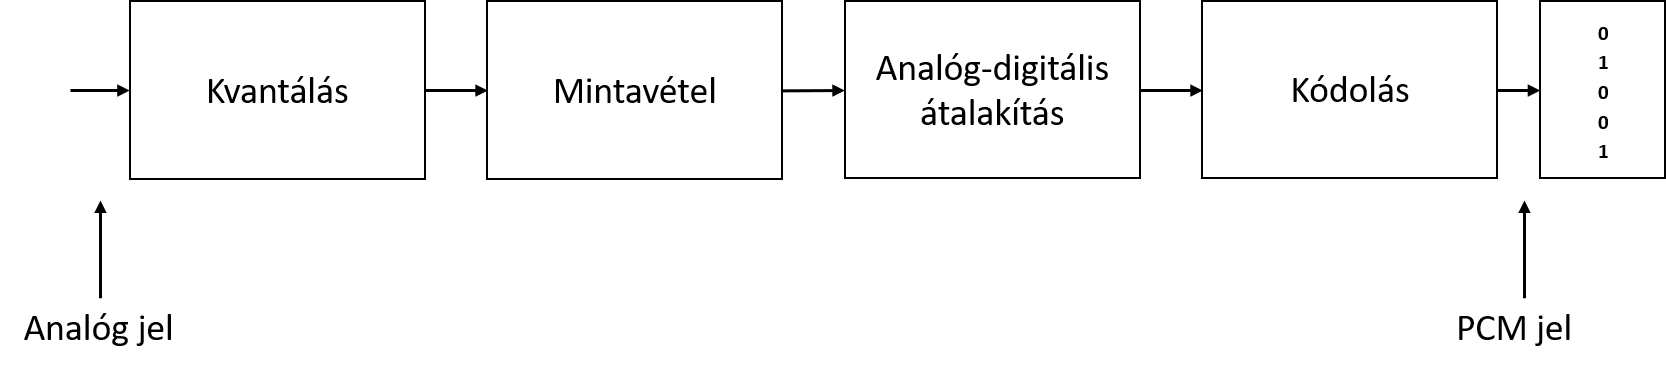
\includegraphics[width=0.7\textwidth]{pcm}
	\caption{A hangdigitalizálás folyamata}
\end{figure}

A digitalizálás első lépése a kvantálás. A kvantálás során a minta felbontását határozzuk meg. Ezek lesznek a kvantálási lépcsők. Minél több részre osztjuk fel az analóg jel feszültségét, annál pontosabban tudjuk rekonstruálni az A/D átalakítás során. A mai hangkártyák 16-24 bit-es (extrém esetekben 64 bites) felbontásokat tudnak produkálni, de a Hifi szabvány szerint a 16 bites felbontás már elegendő az eredeti hang visszaállításához. Ha a folyamatot egy koordináta rendszerben képzeljük el, akkor a sávhatárolás a függőleges tengely beskálázását jelenti a nulla és a maximális feszültségszint között.
A kvantálás, során a feszültségértékek intervallumát felosztjuk véges számú lépésre, és a valós feszültségértékek helyett ezekkel a fix értékekkel számolunk.
\begin{figure}[h]
	\centering
	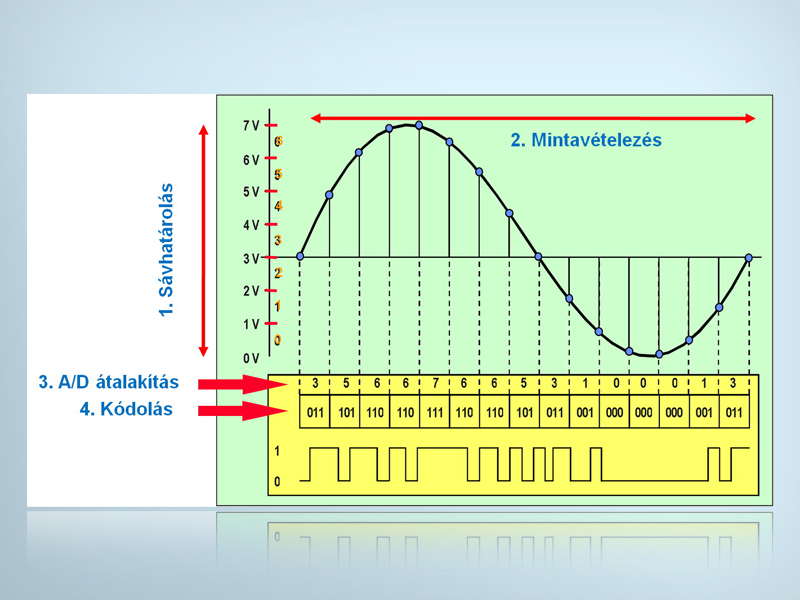
\includegraphics[width=0.7\textwidth]{folyamat}
	\caption{A hangdigitalizálás folyamata}
\end{figure}
\\A digitalizálás második lépése a mintavételezés, ennek során megadott időközönként belemérünk az analóg jelbe, és leolvassuk a feszültséget. Ezek az értékek még nem használhatók digitális feldolgozásra, mivel folytonos információt kapunk. Mintavételezésnél figyelembe kell venni a Shannon-törvényt, amely szerint a jel akkor teljes mértékben visszaállítható, ha a mintavételezési frekvencia a jelben előforduló legnagyobb frekvenciájú összetevőknek legalább a kétszerese. Az emberi hallás frekvenciatartománya 20-20.000 Hz közötti. Magyarul a tétel szerinti legnagyobb frekvencia, ami az analóg jelben előfordul 20.000 Hz. Mivel a tétel szerint legalább ennek a frekvenciának legalább a kétszeresét kell vennünk mintaként, így a mintavételezési frekvencia 40.000 Hz lesz, ami azt jelenti, hogy minimum 40.000 mintát kell vennünk a hangból másodpercenként. A Hifi szabvány szerint a 44.100 Hz, a standard érték, de a profi digitalizálások során az alkalmazott értékek 48 KHz, 96 KHz, 192 KHz is lehetnek. Minél nagyobb ez az érték annál jobb minőséget kapunk. Harmadik lépésben a mintavételezés során vett minták értékeit a digitalizáló algoritmus tárolja, amelyek ebben a fázisban még tízes számrendszerbeli értékek. A kódolás során a hangból vett minták tízes számrendszerbeli pillanatnyi értékeit bináris kódszavakká konvertálódnak. 


\section{Dinamikus idővetemítés}


A Dinamikus idővetemítés egy olyan algormitmus, amely két időbeli szekvencia között(amelyeknek pl. sebessége változhat) hasonlóságot mér. Vegyük például a gyaloglást, dinamikus idővetemítés segítségével ki lehet mutatni a hasonlóságokat, még akkor is ha az egyik személy gyorsabban jár, mint a másik, vagy ha a megfigyelés során gyorsulások és lassulások is voltak.A dinamikus idővetemítést általában video-, audio- és grafikus adatoknak időbeli szekvenciáira szokták alkalmazni, de valójában bármilyen lineáris szekvenciává alakítható adatot lehet elemezni ennek az algoritmusnak a segítségével. Leginkább az automatikus beszédfelismerésben ismert, mert különböző beszédsebességeket tudunk vizsgálni vele. 
\\Általánosságban ez a módszer bizonyos korlátozásokkal és szabályokkal kiszámítja két adott szekvencia közötti optimális egyezést:
\begin{enumerate}
	\item Az első szekvencia minden indexét össze kell egyeztetni egy vagy több indexxel a másik szekvenciából és fordítva is.
	\item Az első szekvenciából az utolsó indexet össze kell egyeztetni az utolsó indexkel a másik szekvenciából (de nem kell az egyetlen egyezésnek lennie).
	\item Az indexek leképezése az első szekvencia és a másik szekvencia indexei között monoton növekszik, és fordítva is. Például, ha j > i indexek az első szekvenciából, akkor nem lehet két index l > k a másik szekvenciából, ahol i index  egyenlő l indexxel és j index egyenlő k indexxel.
	 
\end{enumerate}
Az optimális egyezés az az egyezés, amely megfelel a korlátozásoknak,szabályoknak, amiknek minimális költségük van, és ezeket a költségeket az egyező indexek abszolút különbségeinek összegeként számítják ki.
\\Ezek a szekvenciák nem lineárisan vannak vetemítve az időben, azért hogy meglehessen velük határozni a hasonlóság mértékét, függetlenül az idő bizonyos nem lineáris variációitól. Ezt a fajta szekvencia igazítási módszert gyakran használják az idősorok osztályozásában. 

Az alábbi kód a dinamikus idővetemítés algoritmus implementációját szemlélteti két szekvencia (s és t) esetén, ahol DTW[i, j] a távolság s[1:i] és t[1:j] között.
\begin{figure}[h]
	\centering
	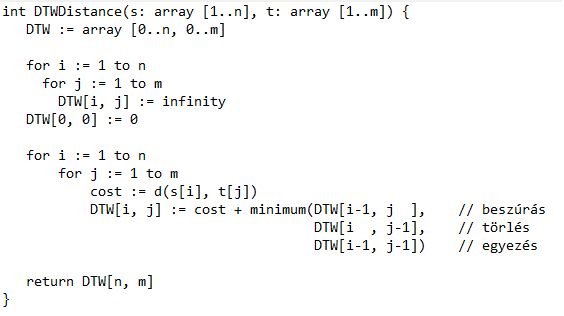
\includegraphics[width=0.7\textwidth]{dtw}
	\caption{Dinamikus idővetemítés implementáció}
\end{figure}
\\Az algoritmus komplexitása O(NM), ahol N és M a két szekvencia hossza.

\section{Rejtett Markov Modell}
\subsection{A modellről általánosan}
A rejtett Markov Modell egy olyan időbeli valószínűségi modell, amelyben a folyamat állapotát egyetlen diszkrét valószínűségi változó írja le.
\\A modell karakterisztikus tulajdonsága a rejtett állapot, azaz a sztochasztikus állapotfejlődés és annak passzív sztochasztikus megfigyelése. Az index időértelmezése helyett bármely szekvenciális értelmezés lehetséges, gyakori például az indexnek mint egy egydimenziós pozíciónak az értelmezése is. A változó lehetséges értékei a világ lehetséges állapotai. Az rejtett Markov modell keretei között további állapotváltozók csak úgy adhatók hozzá az időbeli modellhez, hogy az összes állapotváltozót egyetlen nagy kombináljuk, amelynek az értékei az egyes állapotváltozók értékeinek minden lehetséges kombinációja. Látni fogjuk, hogy a rejtett Markov modellek korlátozott struktúrája lehetővé teszi az összes alapalgoritmus egy nagyon egyszerű és elegáns mátrixos átfordítását.

\subsection{RMM és a beszédfelismerés}
A beszéd jelenti az első találkozásunkat a valódi érzékelők szolgáltatta adatok nyers, tisztítatlan világával. Ezek az adatok zajosak, a szó szoros értelmében: a zaj lehet háttérzaj és lehet a digitalizálási folyamat okozta melléktermék; eltérések lehetnek a szavak kiejtési módjában még ugyanannál a beszélőnél is; különböző szavak hangzása ugyanaz lehet és így tovább. Ezen okok miatt a beszédfelismerésre mint valószínűségi következtetési problémára kezdtek el tekinteni.
\\A legáltalánosabb szinten a valószínűségi következtetési problémát a következőképpen definiálhatjuk. Legyen a Szavak egy valószínűségi változó az összes lehetséges szószekvencia felett, ami elhangozhat, és legyen a jel a megfigyelt akusztikusjel-szekvencia. Ekkor az elhangzottak legvalószínűbb értelmezése a Szavak azon értéke, ami maximalizálja a P(szavak|jel) értéket. Amint az gyakori eset, a Bayes-szabály alkalmazása hasznos:
\\\\
P(szavak|jel) = ALFA P(jel|szavak) P(szavak) 
\\\\
A P(jel|szavak) alkotják az ún. akusztikai modellt (acoustic model). Ez írja le a szavak hangzását – a „ceiling (mennyezet)” egy lágy „c”-vel kezdődik és ugyanúgy hangzik, mint a „sealing (pecsételés/tömítés/fókavadászat)”. (Az azonos hangzású szavakat homofon (homophone) szavaknak nevezzük.) A P(szavak) értékei képezik az ún. nyelvi modellt (language model). Ez adja meg az a priori valószínűségét minden egyes kijelentésnek – például hogy a „magas mennyezet (high ceiling)” sokkal valószínűbb szókapcsolat, mint a „magas pecsételés (high sealing)”.
\\A beszédfelismerő rendszerekben használt nyelvi modellek gyakran igen egyszerűek. A fejezetben később leírt bigram (bigram) modell minden lehetséges esetre megadja annak a valószínűségét, hogy egy szó egy másik szót követ. Az akusztikai modell sokkal bonyolultabb. Az alapjait egy fontos felfedezés alkotja a fonológia (phonology) (a nyelvi hangok tanulmányozása) területéről, nevezetesen, hogy az emberiség minden nyelve egy 40–50 hangból álló korlátos választékkal él, amelyeket beszédhangoknak (phones) hívunk. Egy beszédhang nagyjából az a hang, amely egy egyedi mással- vagy magánhangzónak felel meg. A helyzetet komplikálja valamelyest, hogy az olyan betűkombinációk, mint „th” vagy „ng” egyedi beszédhangot eredményeznek, viszont egyes betűk többféle beszédhanghoz vezetnek, a környezetüktől függően (például az „a” betű a „rat” és a „rate” szóban). A fonéma (phoneme) a legkisebb hangi egység, ami önálló jelentéssel bír egy adott nyelv használói számára. Például az angolban a „t” beszédhang a „stick” szóban ugyanaz a fonéma, mint a „t” beszédhang a „tick” szóban, de a thai nyelvben ezek megkülönböztethetők, mint két különböző fonéma.
\\A beszédhangok létezése lehetővé teszi az akusztikai modell két részre bontását. Az első rész a kiejtést (pronunciation) kezeli, és minden egyes szóra megad egy valószínűség-eloszlást az összes lehetséges beszédhangsor felett. Például a „ceiling” szó kiejtése [s iy l ih ng], vagy néha [s iy l ix ng], vagy esetleg [s iy l en]. A beszédhangok közvetlenül nem megfigyelhetők, így nagyjából a beszéd egy olyan rejtett Markov-modellel reprezentálható, aminek Xt állapotváltozója a t időpontban kimondott beszédhang.
\\Az akusztikai modell második része a beszédhangok akusztikus jelként való megvalósulási módjával foglalkozik: azaz a rejtett Markov-modell Et bizonyítékváltozója adja meg az akusztikus jel t időpontban megfigyelt jellemzőit, és az akusztikus modell adja meg az P(Et|Xt) feltételes valószínűséget, ahol Xt az aktuális beszédhang. A modellnek lehetőséget kell adni eltérésekre a hangmagasságban, a sebességben és a hangerőben, és jelfeldolgozási (signal processing) technikákon alapul, hogy olyan jelreprezentációt biztosítson, ami megfelelően robusztus módon kezeli ezeket a fajta eltéréseket.
\\Beszéd esetén a tipikus mintavételi frekvencia 8 és 16 kHz (azaz 8000-től 16 000-ig másodpercenként) között van. (Jó minőségű zenei felvételeket mintavételeznek 44 kHz vagy még magasabb frekvenciával.) A mérés pontosságát az egyes mintavételi pontokban a kvantálási tényező (quantization factor) határozza meg; a beszédfelismerők tipikusan 8–12 bitet használnak. Ez azt jelenti, hogy a legkevésbé igényes rendszer, amely 8 kHz-es frekvenciával mintavételez, és 8 bites kvantálást használ, közel fél megabájtot igényel egy egyperces beszéd tárolásához. Ilyen nagy mennyiségű jelinformáció esetén kivitelezhetetlen létrehozni és használni a P(jel|beszédhang) eloszlásokat, így az akusztikus jelnek tömörebb leírásait kell kifejlesztenünk.
\\Elsőként azt vesszük figyelembe, hogy bár a beszédben a hangfrekvencia akár több kHz-es is lehet, a jel tartalmának a megváltozásai sokkal ritkábban fordulnak elő, talán nem több mint 100 Hz-cel. Ezért a beszédrendszerek a jel tulajdonságait hosszabb időintervallumonként, úgynevezett keretenként (frames) összegzik. Egy 10 ms-os (80 minta 8 kHz-es mintavétel mellett) keret elég rövidnek tűnik ahhoz, hogy csak néhány rövid idejű jelenség mosódjon el az összegzési folyamat miatt. Az egyes kereteken belüli folyamatot egy jellemző (feature) vektorral ábrázoljuk. Például jellemezni akarjuk az energia szintjét számos frekvenciasáv mindegyikében. Más fontos jellemzők a keret globális energiaszintje és a megelőző kerettől számított (energia)különbség. A jellemzők kiemelése a beszédjelből hasonlít egy kicsit arra, ahogy a zenekar játékát figyelve megjegyezzük: „Most a vadászkürtök hangosan és a hegedűk halkan szólnak.” .Figyeljük meg az alábbi ábrán, hogy a keretek átlapolódnak; ez megvéd minket attól, hogy pont a keret határán fellépő fontos akusztikus események információját elveszítsük.
\begin{figure}[h]
	\centering
	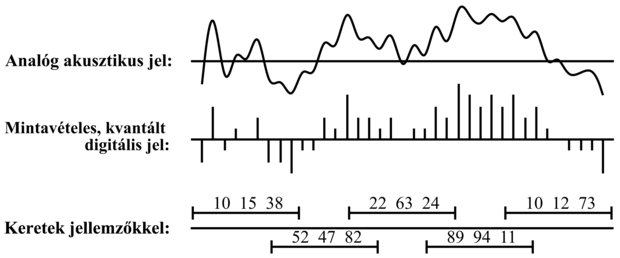
\includegraphics[width=0.7\textwidth]{folyamat2}
	\caption{Az átalakítás lépései a nyers hangtól a keretek sorozatáig.
	}
\end{figure}
\\A példánkban csupán három jeggyel rendelkező keretet mutattunk. Valós rendszerek jellemzők tucatjaival vagy akár százaival dolgoznak. Például n darab jellemző esetén, amikor mindegyik 256 lehetséges értéket vehet fel, egy keret egy ponttal adható meg egy n-dimenziós térben, és 256n lehetséges keret létezik. n > 2 esetén kivitelezhetetlen volna a P(jellemzők|beszédhang) eloszlásnak egy explicit táblázatként történő ábrázolása, így további tömörítésre van szükségünk. Két lehetséges megközelítés létezik:

	\begin{enumerate}
		\item	A vektorkvantálás (VK) (vector quantization, VQ) módszere felosztja az n dimenziós teret mondjuk 256 partícióra, C1-től C256-ig címkézve. Ekkor az egyes kereteket inkább egy egyedi címkével, mint egy n számból álló vektorral lehet jellemezni. Így a P(VQ|beszédhang) eloszlás táblázatos formája 256 valószínűséget tartalmaz minden egyes beszédhangra. Nagy rendszerekben a vektorkvantálás már nem népszerű.
		\item A jellemzők terének diszkretizálása helyett parametrikus folytonos eloszlásokat használhatunk a P(jellemzők|beszédhang) leírásához. Például használhatunk minden beszédhanghoz egy Gauss-eloszlást, beszédhangonként különböző átlaggal és kovarianciamátrixszal. Ez jól működik, ha az egyes beszédhangok akusztikus megvalósulása a jellemzők terében egyetlen területen csoportosul. A gyakorlatban egy hanghoz több területen való csoportosulás is tartozik, és Gauss-eloszlások keverékét (mixture of Gaussians) kell használni. Egy keverék k egyedi eloszlás súlyozott összege, így a P(jellemzők|beszédhang) eloszláshoz k súly, k n elemű átlagvektor és k n2 méretű kovarianciamátrix tartozik, ami O(kn2) paraméter minden beszédhangra.
	\end{enumerate}


Természetesen bizonyos információ elvész a feldolgozás során, ami a teljes beszédjeltől egy VK címkéig vagy a keverékparaméterek egy halmazáig tart. A jelfeldolgozás művészete abban rejlik, hogy úgy válasszuk meg a jellemzőket és a tartományokat (vagy a Gauss-eloszlásokat), hogy a hasznos információ vesztesége minimális legyen. Egy adott beszédhang számos módon kiejthető: hangosan vagy halkan, gyorsan vagy lassan, magasan vagy mély hangon, csendben vagy háttérzajban és beszélők sok milliója által, mindegyikőjük különböző kiejtésével és eltérő hangképző szerveivel.
\\Még két további finomítást kell elvégeznünk az eddig leírt egyszerű modellen. Az első a beszédhangok időbeli szerkezetével foglalkozik. Normális beszédben a legtöbb beszédhangnak a terjedelme 50–100 ezredmásodperc vagy 5–10 keret. A P(jellemzők|beszédhang) valószínűségi modell ugyanaz ezen keretek mindegyikére, pedig a legtöbb beszédhangnak jelentős belső struktúrája van. Például a [t] egyike a zárhangoknak (stop consonants), amelyekben a levegő áramlása megszűnik egy rövid időre egy határozott kibocsátás előtt. Az akusztikus jelet megvizsgálva azt látjuk, hogy egy [t]-nek a kezdete hangtalan, közepén egy kis kirobbanással és (általában) egy sziszegéssel a végén. A beszédhangoknak ez a belső struktúrája egy háromállapotú modellel ragadható meg; minden beszédhangnak van egy kezdeti, közép- és végállapota, és minden állapotnak megvan a saját eloszlása a jegyek felett.
\\A második finomítás azzal a környezettel foglalkozik, amelyben a beszédhang elhangzik. Egy adott beszédhang hangzását megváltoztathatják a környező beszédhangok. Emlékezzünk arra, hogy a beszédhangok az ajkak, a nyelv és az álkapocs mozgása és a levegőnek a hangképző szerveken történő kényszerített átáramlása révén keletkezik. Ezen komplex mozgások koordinálásánál, amik másodpercenként öt vagy még több beszédhangot produkálnak, az agy már akkor elindít a második beszédhanghoz tartozó műveletet, mielőtt az első befejeződött volna, így megváltoztatva az egyik vagy mindkét beszédhangot. Például a „sweet (édes)” kiejtésénél az ajkak kerekítettek az [s] előállítása közben számítva a következő [w]-re. Ezeket a koartikulációs hatásokat (coarticulation effects) részlegesen megragadja a hármashangzó (triphone) modell, amelyben az egyes beszédhangok akusztikai modellje függhet az előző és következő beszédhangtól. Így a [w] a „sweet”-ben úgy írható, hogy [w(s,iy)], azaz [w] egy [s] bal- és egy [iy] jobb-környezetben.
\\ A háromállapotú és hármashangzó modellek együttes hatása megnöveli az időbeli folyamat lehetséges állapotainak a számát az eredeti beszédhang készletbeli n beszédhangról 3n3-ra (az ARPAbet-ben n kozelitoleg 50). A tapasztalatok azt mutatják, hogy a megnövelt pontosság bőven ellensúlyozza a következtetés és a tanulás megnövekedett költségeit.


\section{Elérhető szoftveres eszközök áttekintése}


\subsection{CMU Sphinx}
% https://pypi.org/project/pocketsphinx/

A CMU Sphinx egy beszédfelismerő rendszerek csoportja, amelyet a Carnegie Mellon Egyetemen fejlesztenek. Első verziója a Sphinx melyet Kai-Fu Lee hozott létre , egy folyamatos beszédfelismerő rendszer, amely rejtett markov modellt és n-gram statisztikai nyelvi modellt használ. Azóta számos verziója jött ki ennek a programnak, melyek sokkal nagyobb hatékonysággal működnek. Érdemes megemlíteni a PocketSphinx változatot, mely beágyazott rendszerekre lett optimizálva. 

\subsection{Praat}

A Praat szintén egy beszédfelismerő rendszer, de ez inkább a fonetikai beszéd tudományos elemzésére készült.


\section{Szavak szegmentálása és felismerése}
Minden egyes szóra gondolhatunk úgy, mint ami meghatároz egy külön P($X_{1:t}$|szó) valószínűségi eloszlást, ahol $X_{i}$ megadja az i-edik keretben a beszédhang állapotát. Tipikusan ezt az eloszlást két részre osztjuk. A kiejtési modell (pronunication model) egy eloszlást ad meg a beszédhangsorok felett (figyelmen kívül hagyva az ütemet és a kereteket), majd a beszédhangmodell (phone model) leírja, ahogyan a beszédhangok leképződnek a keretek szekvenciájára.
\\Gondoljunk arra a szóra, hogy „tomato (paradicsom)”. Gershwin szerint ezt úgy ejtik ki, hogy [t ow m ey t ow] (Gershwin, 1937), én viszont úgy ejtem, hogy [t ow m aa t ow]. A 6. ábra felső részén látható egy olyan állapotátmenet-modell, ami gondoskodik erről a változatról. A modellen keresztül csak két út létezik, egy, ami a [t ow m ey t ow] beszédhang szekvenciához tartozik, és a másik a [t ow m aa t ow] szekvenciához. Egy út valószínűsége az útvonalat alkotó nyilakon szereplő valószínűségek szorzata:
\\ P([towmeytow]|„tomato”) = P([towmaatow]|„tomato”) = 0,5 
\\A fonetikai változékonyság második forrása a koartikuláció (coarticulation). Például a [t] beszédhangnál a nyelv a szájpadlásnál helyezkedik el, az [ow]-nál viszont a száj alján. Gyors beszédnél a nyelv sokszor közbülső pozícióba kerül, melynek eredménye inkább a [t ah], és nem a [t ow]. A 6. ábra alsó része a „tomato” kiejtésének egy bonyolultabb modelljét mutatja, amely ezt a koartikulációs hatást figyelembe veszi. Ebben a modellben négy különböző út van, és azt kapjuk, hogy:
\\P([towmeytow]|„tomato”) = P([towmaatow]|„tomato”) = 0,1
\\
\\P([tahmeytow]|„tomato”) = P([tahmaatow]|„tomato”) = 0,4 
\\A háromállapotú beszédhangmodell állapotátmenet-diagramja a 7. ábrán látható. A modell egy konkrét beszédhanghoz tartozik, az [m]-hez, de az összes beszédhangnak hasonló topológiájú modellje van. Az ábrán láthatók az egyes beszédhang állapotokhoz kapcsolódó akusztikai modellek is, feltételezve, hogy a jelet egy VK címke reprezentálja. Például a modell szerint P(Et = C1|Xt = [m]Kezdet) = 0,5. Vegyük észre a hurkokat az ábrán; például az [m]Közép állapot 0,9 valószínűséggel fennmarad, ami azt jelenti, hogy az [m]Közép állapot várható időtartama 10 keret. A modellünkben az egyes beszédhangok hossza független a többi beszédhang hosszától; egy kifinomultabb modell képes lenne a gyors és lassú beszédet megkülönböztetni.
\\Hasonló modelleket hozhatunk létre minden egyes beszédhangra, akár a hármashangzó környezet hatását is figyelembe véve. Minden szómodell, amikor a beszédhangmodellekkel kombináljuk, egy RMM teljes specifikációját adja. A modell megadja a beszédhang állapotok közötti, keretről keretre történő átmeneteknek a valószínűségeit csakúgy, mint az akusztikus jegyek valószínűségeit minden egyes beszédhang állapothoz.
\begin{figure}[h]
	\centering
	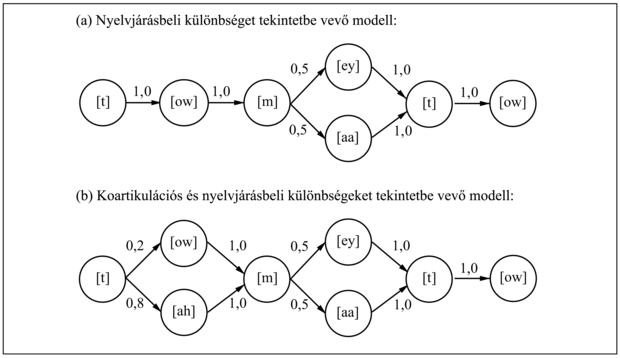
\includegraphics[width=0.7\textwidth]{szavak1}
	\caption{A „tomato” szó két kiejtési modellje. Mindegyik modellt egy átmenetdiagramként ábrázoljuk, amiben az állapotokat körrel jelöljük, a megengedett átmeneteket pedig nyilakkal, rajtuk a kapcsolódó valószínűségekkel. (a) Egy nyelvjárásbeli különbségeket is tekintetbe vevő modell. A 0,5-ös értékek a két szerző preferált kiejtésein alapuló becslések. (b) Egy olyan modell, ami az első magánhangzón egy koartikulációs hatást is figyelembe vesz, megengedve az [ow] vagy az [ah] beszédhangokat.
	}
\end{figure}
\newpage
\begin{figure}[h]
	\centering
	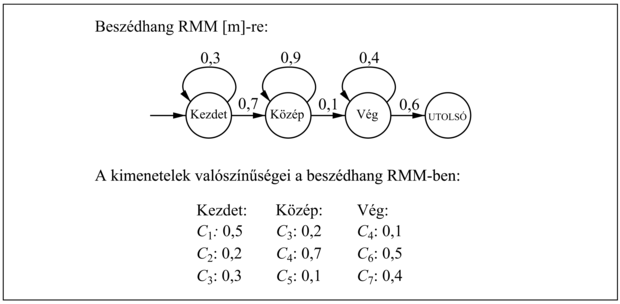
\includegraphics[width=0.7\textwidth]{szavak2}
	\caption{Az [m] háromállapotú beszédhang egy RMM-je. Mindegyik állapotnak számos lehetséges kimenetele lehet, különálló valószínűségekkel. A C1, …, C7 VK-címkék önkényesen lettek megválasztva.}
\end{figure}
Ha egyedülálló szavakat (isolated words) szeretnénk felismerni – azaz egyértelmű határokkal rendelkező és mindennemű környezeti összefüggés nélkül kiejtett szavakat –, akkor azt a szót kell megkeresnünk, amelyik maximalizálja azt, hogy:
\\ P(szó|e1:t) = alfaP(e1:t|szó)P(szó) 
A P(szó) a priori valószínűség valódi szöveges adatból kapható meg. A P(e1:t|szó) pedig az akusztikus jegyek sorozatának a valószínűsége a szómodell szerint. 



\end{document}
